% Spellcheck: ok
% Mikes: ok

\chapter{Intermezzo: Mythbusting�Bigfoot, Least Squares, and All That}{}{}
\label{ch:bigfoot}

\Fint{Everybody has heard of Bigfoot, the mystical figure that lives in the
woods, but nobody has ever} actually seen him. Similarly, there are
some concepts from basic statistics that everybody has heard of but
that---like Bigfoot---always remain a little shrouded in mystery.
Here, we take a look at three of them: the average of averages, the
mystical standard deviation, and the ever-popular least squares.

\vspace*{-6pt}
% ============================================================
\section{How to Average Averages}

\index{averaging averages|(} 

Recently, someone approached me with the following question: given the
numbers in Table \ref{tbl:avgaverages}, what number should be entered
in the lower-right corner? Just adding up the individual defect rates
per item and dividing by 3 (in effect, averaging them) did not seem
right---if only because it would come out to about $0.75$, which is
pretty high when one considers that \emph{most} of the units produced
(100 out of 103) are not actually defective. The specific question
asked was: ``Should I weight the individual rates somehow?''

\begin{table}
\vspace*{-6pt}
\def\a{\hphantom{0}}
\def\vrl{\smash{\vrule height43.8pt  width.25pt depth5pt}}
\def\vvrl{\smash{\vrule height58.6pt  width.25pt depth5pt}}
\tbl{Defect rates: what value should go into the lower-right
  corner?\label{tbl:avgaverages}}{%
\begin{tabular}{c@{\hskip9pt}c@{\hskip9pt}c@{\hskip9pt}c@{\hskip9pt}c@{\hskip9pt}c@{\hskip9pt}c}
\toprule
\TCH{Item type}   & & \TCH{Units produced} &&\TCH{Defective units} && \TCH{Defect rate} \\\colrule
A         && \a\a2              && 1               && 0.5\a  \\
B         && \a\a1              && 1               && 1.0\a \\
C         &\vrl& 100            &\vrl& 1               && 0.01 \\\colrule
\multicolumn{5}{l}{\textbf{Total defect rate}}   &\vvrl& \textbf{???}  \\
\botrule
\end{tabular}}
\end{table}

This situation comes up frequently but is not always recognized: we
have a set of rates (or averages) and would like to summarize them\vadjust{\pagebreak}
into an overall rate (or overall average). The problem is that the
naive way of doing so (namely, to add up the individual rates and then
to divide by the number of rates) will give an \emph{incorrect}
result.  However, this is rarely noticed unless the numbers involved
are as extreme as in the present example.

The correct way to approach this task is to start from scratch.  What
is the ``defect rate,'' anyway? It is the number of defective items
divided by the number of items produced. Hence, the \emph{total}
defect rate is the total number of defective items divided by the
total number of items produced: $3/103 \approx 0.03$.  There should be
no question about that.

Can we arrive at this result in a different way by starting with the
individual defect \emph{rates}? Absolutely---provided we weight them
appropriately. Each individual defect rate should contribute to the
overall defect rate in the same way that the corresponding item type
contributes to the total item count. In other words, the weight for
item type A is $2/103$, for B is $1/103$, and for C it is $100/103$.
Pulling all this together, we have: $0.5 \cdot 2/103 + 1.0 \cdot 1/103
+ 0.01 \cdot 100/103 = (1+1+1)/103 = 3/103$ as before.

To show that this agreement is not accidental, let's write things out
in greater generality:\vspace*{-2pt}
%
\begin{align*}
n_k & \qquad \text{Number of items of type $k$} \\
d_k & \qquad \text{Number of defective items of type $k$} \\
\epsilon_k = \frac{d_k}{n_k} & \qquad \text{Defect rate for type $k$} \\
f_k = \frac{n_k}{\sum_i n_i} & \qquad 
  \text{Contribution of type $k$ to total production} 
\end{align*}
%
Now look at what it means to weight each individual defect rate:\vspace*{-2pt}
%
\begin{align*}
f_k \epsilon_k & = \frac{n_k}{\sum_i n_i} \frac{d_k}{n_k} \\
 & = \frac{d_k}{\sum_i n_i}
\end{align*}
%
In other words, weighting the individual defect rate $\epsilon_k$ by
the appropriate weight factor $f_k$ has the effect of turning the
defect \emph{rate} back to the the defect \emph{count} $d_k$
(normalized by total number of items).

In this example, each item could get only one of two ``grades,''
namely $1$ (for defective) or $0$ (for not defective), and so the
``defect rate'' was a measure of the ``average defectiveness'' of a
single item. The same logic as just demonstrated applies if you have a
greater (or different) range of values. (You can make up your own
example: give items grades from $1$ to $5$, and then calculate the
overall ``average grade'' to see how it works.)

\vspace*{-6pt}
\subsection{Simpson's Paradox}

\index{Simpson's paradox}
 
Since we are talking about mystical figures that can sometimes be
found in tables, we should also mention \emph{Simpson's paradox}. Look
at Table \ref{tbl:simpson} which shows applications and admissions to
a fictional college in terms the applicants' gender and department.\pagebreak

\begin{table}
\def\a{\hphantom{0}}
\def\vrl{\smash{\vrule height48.6pt  width.25pt depth5pt}}
\tbl{Simpson's paradox: applications and admissions 
  by gender of applicant.\label{tbl:simpson}}{%
\begin{tabular}{l@{\hskip9pt}c@{\hskip9pt}c@{\hskip9pt}c@{\hskip9pt}c@{\hskip9pt}c@{\hskip9pt}c}\toprule
 && \TCH{Male} & & \TCH{Female} &&\TCH{Overall} \\\colrule
Department A    && 80/100 $=$ 0.8\hphantom{0}  && $\hphantom{00}$9/10 $=$ 0.9\hphantom{0}    && 89/110 $=$ 0.81 \\
Department B    && $\hphantom{00}$5/10 $=$ 0.5\hphantom{0}  && 60/100 $=$ 0.6\hphantom{0}    && 65/110 $=$ 0.59\hspace*{1.2pt}\\\colrule
\textbf{Total}  &\vrl& {\bfseries 85}$\mathbf{/}${\bfseries 110} $\mathbf{=}$ {\bfseries 0.77} &\vrl& {\bfseries 69}$\mathbf{/}${\bfseries
110} $\mathbf{=}$ {\bfseries 0.63} &\vrl&
\\\botrule
\end{tabular}}
\end{table}

If you look only at the bottom line with the totals, then it might
appear that the college is discriminating against women, since the
acceptance rate for male applicants is higher than that for female
applicants (0.77 versus 0.63).\footnote{You should check that the
  entries in the bottom row have been calculated properly, per the
  discussion in the previous section!}  But when you look at the rates
for each individual department within the college, it turns out that
women have \emph{higher} acceptance rates than men for \emph{every}
department.  How can that be?

The short and intuitive answer is that many more women apply to
department B, which has a lower overall admission rate than department
A (0.59 versus 0.81), and this drags down their (gender-specific)
acceptance rate. 

The more general explanation speaks of a ``reversal of association \index{reversal of association} due
to a confounding factor.'' When considering only the totals, it may
seem as if there is an association between gender and admission rates,
with male applicants being accepted more frequently.  However, this
view ignores the presence of a hidden but important factor: the choice
of department. In fact, the choice of department has a \emph{greater}
influence on the acceptance rate than the original explanatory
variable (the gender).  By lumping the observations for the different
departments into a single number, we have in fact masked the influence
of this factor---with the consequence that the association between
acceptance rate (which favors women for each department) and gender
was reversed.

The important insight here is that such ``reversal of association''
due to a confounding factor is always possible. However, both
conditions must occur: the confounding factor must be sufficiently
strong (in our case, the acceptance rates for departments A and B were
sufficiently different), and the assignment of experimental units to
the levels of this factor must be sufficiently imbalanced (in our
case, many more women applied to department B than to department A).
% In fact, one can work out conditions for the minimum strength that a
% confounding factor must have to bring about a reversal of association
% (such as ``Cornfield's Condition'').

As opposed to Bigfoot, Simpson's paradox is known to occur in the
real world. The example in this section, for instance, was based on a
well-publicized case involving the University of California (Berkeley)
in the early 1970s. A quick Internet search will turn up additional
examples.

\index{averaging averages|)} 

% ============================================================
\section{The Standard Deviation}

\index{standard deviation|(} 

The fabled standard deviation is another close relative of Bigfoot.
Everybody (it seems) has heard of it, everybody knows how to calculate
it, and---most importantly---everybody knows that 68 percent of all data
points fall within 1 standard deviation, 95 percent within 2, and
virtually all (that is: 99.7 percent) within 3.

Problem is: this is utter nonsense. 

It is true that the standard deviation is a measure for the spread (or
width) of a distribution. It is also true that, for a given set of
points, the standard deviation can always be calculated. But that does
not mean that the standard deviation is always a \emph{good} or
appropriate measure for the width of a distribution; in fact, it can
be quite misleading if applied indiscriminately to an unsuitable data
set. Furthermore, we must be careful how to interpret it: the whole 68
percent business applies only if the data set satisfies some very
specific requirements.

In my experience, the standard deviation is probably the most
misunderstood and misapplied quantity in all of statistics.

Let me tell you a true story (some identifying details have been
changed to protect the guilty). The story is a bit involved, but this
is no accident: in the same way that Bigfoot sightings never occur in
a suburban front yard on a sunny Sunday morning, severe
misunderstandings in mathematical or statistical methods usually don't
reveal themselves as long as the applications are as clean and simple
as the homework problems in a textbook. But once people try to apply
these same methods in situations that are a bit less standard,
\emph{anything} can happen. This is what happened in this particular
company.

I was looking over a bit of code used to identify outliers in the
response times from a certain database server. The purpose of this
program was to detect and report on uncommonly slow responses.  The
piece of code in question processed log files containing the response
times and reported a threshold value: responses that took longer than
this threshold were considered ``outliers.''

An existing service-level agreement defined an outlier as any value
``outside of 3 standard deviations.''  So what did this piece of code
do? It sorted the response times to identify the top 0.3 percent of
data points and used those to determine the threshold. (In other
words, if there were 1,000 data points in the log file, it reported
the response time of the third slowest as threshold.)  After all, 99.7
percent of data points fall within 3 standard deviations. Right?

After reading Chapter \ref{ch:univariate}, I hope you can immediately
tell where the original programmer went wrong: the threshold that the
program reported had \emph{nothing at all} to do with standard
deviations---instead, it reported the top 0.3 percentile.  In other
words, the program completely failed to do what\vadjust{\pagebreak} it was supposed to do.
Also, keep in mind that it is incorrect to blindly consider the top
$x$ percent of any distribution as outliers (review the discussion of
box plots in Chapter \ref{ch:univariate} if you need a reminder).

But the story continues. This was a database server whose typical
response time was less than a few seconds. It was clear that anything
that took longer than one or two minutes had to be considered
``slow''---that is, an outlier. But when the program was run, the
threshold value it reported (the 0.3 percentile) was on the order of
\emph{hours}.  Clearly, this threshold value made no sense.

In what must have been a growing sense of desperation, the original
programmer now made a number of changes: from selecting the top 0.3
percent, to the top 1 percent, then the top 5 percent and finally the
top 10 percent. (I could tell, because each such change had dutifully
been checked into source control!) Finally, the programmer had simply
hard-coded some seemingly ``reasonable'' value (such as 47 seconds or
something) into the program, and that's what was reported as ``3
standard deviations'' regardless of the input.

It was the only case of outright technical fraud that I have ever
witnessed: a technical work product that---with the original author's
full knowledge---in no way did what it claimed to do.

What went wrong here? Several things. First, there was a fundamental
misunderstanding about the definition of the standard deviation, how
it is calculated, and some of the properties that in practice it often
(but not always) has. The second mistake was applying the standard
deviation to a situation where it is not a suitable measure.

Let's recap some basics: we often want to characterize a point
distribution by a typical value (its location) and its spread around
this location.  A convenient measure for the location is the mean:
$\mu = \frac{1}{n} \sum_i^n x_i$. Why is the mean so convenient?
Because it is easy to calculate: just sum all the values and divide by
$n$.

To find the width of the distribution, we would like see how far
points ``typically'' stray from the mean. In other words, we would
like to find the \emph{mean} of the \emph{deviations} $x_i - \mu$. But
since the deviations can be positive and negative, they would simply
cancel, so instead we calculate the mean of the \emph{squared}
deviations: $\sigma^2 = \frac{1}{n} \sum_i^n \paren{x_i - \mu}^2$.
This quantity is called the \emph{variance}, and its square root is
the \emph{standard deviation}. Why do we bother with the square root?
Because it has the same units as the mean, whereas in the variance the
units are raised to the second power.

Now, \emph{if and only if} the point distribution is well behaved
(which in practice means: it is Gaussian), \emph{then} it is true that
about 68 percent of points will fall within the interval $[\mu -
\sigma, \mu + \sigma]$ and that 95 percent fall within the interval
$[\mu - 2\sigma, \mu + 2\sigma]$ and so on.  The inverse is \emph{not}
true: you cannot conclude that 68 percent of points define a
``standard deviation'' (this is where the programmer in our story made
the first mistake). If the point distribution is not Gaussian, then
there are no particular patterns by which fractions of points will
fall within 1, 2, or any number of standard deviations from the mean.
However, keep in mind that the definitions of\vadjust{\pagebreak} the mean and the
standard deviation (as given by the previous equations) both retain
their meaning: you can calculate them for any distribution and any
data set.

However (and this is the second mistake that was made), if the
distribution is strongly asymmetrical, then mean and standard
deviation are no longer good measures of location and spread,
respectively. You can still \emph{calculate} them, but their values
will just not be very informative. In particular, if the distribution
has a fat tail then both mean and standard deviation will be
influenced heavily by extreme values in the tail.

In this case, the situation was even worse: the distribution of
response times was a \emph{power-law} distribution, which is extremely
poorly summarized by quantities such as mean and standard deviation.
This explains why the top 0.3 percent of response times were on the
order of hours: with power-law distributions, all values---even
extreme ones---can (and do!) occur; whereas for Gaussian or
exponential distributions, the range of values that do occur in
practice is pretty well limited. (See Chapter \ref{ch:probability} for
more information on power-law distributions.)

To summarize, the standard deviation, defined as $\sqrt{\frac{1}{n}
  \sum_i^n \paren{x_i - \mu}^2}$, is a measure of the width of a
distribution (or a sample). It is a good measure for the width only if
the distribution of points is well behaved (\ie, symmetric and without
fat tails).  Points that are far away from the center (compared to the
width of the distribution) can be considered outliers. For
distributions that are less well behaved, you will have to use other
measures for the width (\eg, the inter-quartile range); however, you
can usually still identify outliers as points that fall outside the
typical range of values. (For power-law distributions, which do not
have a ``typical'' scale, it doesn't make sense to define outliers by
statistical means; you will have to justify them differently---for
instance by appealing to requirements from the business domain.)


\subsection{How to Calculate}

Here is a good trick for calculating the standard deviation
efficiently.  At first, it seems you need to make two passes over the
data in order to calculate both mean and standard deviation. In the
first pass you calculate the mean, but then you need to make a second
pass to calculate the deviations from that mean:
%
\[
\sigma^2 = \frac{1}{n} \sum \paren{ x_i - \mu }^2 
\]
%
It appears as if you can't find the deviations until the mean $\mu$
is known.

However, it turns out that you can calculate both quantities in a
single pass through the data. All you need to do is to maintain both
the sum of the values ($\sum x_i$) and the sum of the squares of the
values ($\sum x_i^2$), because\vadjust{\pagebreak} you can write the preceding equation
for $\sigma^2$ in a form that depends only on those two sums:
\begin{align*}
\sigma^2 & = \frac{1}{n} \sum \paren{ x_i - \mu }^2 \\
         & = \frac{1}{n} \sum \paren{ x_i^2 - 2 x_i \mu + \mu^2 } \\
         & = \frac{1}{n} \paren{\sum x_i^2 - 2 \mu \sum x_i + \mu^2 \sum 1} \\
         & = \frac{1}{n} \sum x_i^2 - 2 \mu \frac{1}{n} \sum x_i 
                + \mu^2 \frac{1}{n} n \\
         & = \frac{1}{n} \sum x_i^2 - 2 \mu \cdot \mu + \mu^2 \\
         & = \frac{1}{n} \sum x_i^2 - \mu^2 \\
         & = \frac{1}{n} \sum x_i^2 - \paren{\frac{1}{n} \sum x_i}^2
\end{align*}

This is a good trick that is apparently too little known. Keep it in 
mind; similar situations crop up in different contexts from time to
time.
% The typical size of a random walk, or of an isolated polymer chain in
% solution is calculated in a a way which follows \emph{exactly} the
% same argument, for instance.
(To be sure, the floating-point properties of both methods are
different, but if you care enough to worry about the difference, then
you should be using a library anyway.)


\subsection{Optional: One over What?}

% larsen/marx, p383ff

You may occasionally see the standard deviation defined with an $n$ in
the denominator and sometimes with a factor of $n-1$ instead. 
%
\[
\sqrt{\frac{1}{n} \sum_i^n \paren{ x_i - \mu }^2 }
\qquad \text{or} \qquad
\sqrt{\frac{1}{n-1} \sum_i^n \paren{ x_i - \mu }^2 }
\]
%
What \emph{really} is the difference, and which expression should you
use?

The factor $1/n$ applies only if you know the exact value of the mean
$\mu$ ahead of time. This is usually not the case; instead, you will
usually have to calculate the mean from the data.  This adds a bit of
uncertainty, which leads to the widening of the proper estimate for
the standard deviation. A theoretical argument then leads to the use
of the factor $1/(n-1)$ instead of $1/n$.

In short, if you calculated the mean from the data (as is usually the
case), then you should really be using the $1/(n-1)$ factor. The
difference is going to be small, unless you are dealing with very
small data sets.

\subsection{Optional: The Standard Error}

\index{standard error!about} 

While we are on the topic of obscure sources of confusion, let's talk
about the \emph{standard error}.

The standard error is the standard deviation of an estimated quantity.
Let's say we estimate some quantity (\eg, the mean). If we repeatedly
take samples, then the means calculated from those samples will
scatter around a little, according to some distribution. The standard
deviation of this distribution is the ``standard error'' of the
estimated quantity (the mean, in this example).

The following observation will make this clearer.  Take a sample of
size $n$ from a normally distributed population with standard
deviation $\sigma$. Then 68 percent of the members of the
\emph{sample} will be within $\pm \sigma$ from the estimated mean
(\ie, the sample mean).

However, the mean itself is normally distributed (because of the
Central Limit Theorem, since the mean is a sum of random variables)
with standard deviation $\sigma/\sqrt{n}$ (again because of the
Central Limit Theorem).  So if we take several samples, each of size
$n$, then we can expect 68 percent of the estimated means to lie
within $\pm \sigma/\sqrt{n}$ of the \emph{true} mean (\ie, the mean of
the overall population).

In this situation, the quantity $\sigma/\sqrt{n}$ is therefore the
\emph{standard error of the mean}.

\index{standard deviation|)} 

% ============================================================
\section{Least Squares}

\index{least squares|(} 

Everyone loves least squares. In the confusing and uncertain world of
data and statistics, they provide a sense of security---something to
rely on! They give you, after all, the ``best'' fit.  Doesn't that say
it all?

\begin{figure}
  \centerline{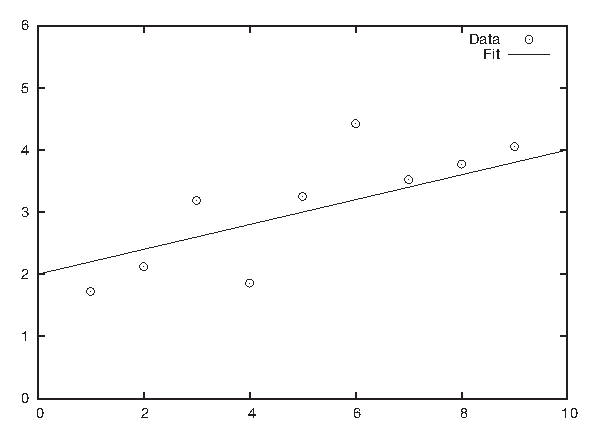
\includegraphics{img/bigfootfit1}}
  \caption{Fitting for statistical parameter estimation: data affected
    by random noise. What is the slope of the straight line?}
  \label{fig:bigfoot1}\vspace*{-6pt}
\end{figure}

Problem is, I have \emph{never} (not once!) seen least squares applied
appropriately, and I have come to doubt that it should ever be
considered\vadjust{\pagebreak} a suitable technique.  In fact, when today I see someone
doing anything involving ``least-squares fitting,'' I am pretty
certain this person is at wit's end---and probably does not even know
it!

There are two problems with least squares. The first is that it is
used for two very different purposes that are commonly confused. The
second problem is that least-squares fitting is usually not the best
(or even a suitable) method for either purpose. Alternative techniques
should be used, depending on the overall purpose (see first problem)
and on what, in the end, we want to do with the result.

Let's try to unravel these issues.

Why do we ever want to ``fit'' a function to data to begin with? There
are two different reasons.

\begin{unnumlist}
\subparagraph{Statistical Parameter Estimation}\vspace*{3pt}
Data is corrupted by random
  noise, and we want to extract parameters from it. \index{statistical parameter estimation}
\subparagraph{Smooth Interpolation or Approximation}\index{smoothing!least squares}
\index{interpolation, least squares} \index{approximations, function approximation with least
squares}\vspace*{3pt}
Data is given as
  individual points, and we would like either to find a smooth
  interpolation to arbitrary positions between those points or to
  determine an analytical ``formula'' describing the data.
\end{unnumlist}

These two scenarios are conceptually depicted in Figures
\ref{fig:bigfoot1} and \ref{fig:bigfoot2}.

\begin{figure}
  \centerline{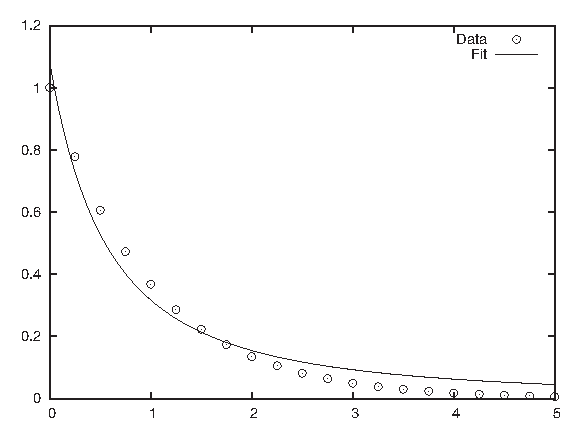
\includegraphics{img/bigfootfit2}}
  \caption{Fitting a function to approximate a curve known only at 
    discrete locations. Is the fit a good representation of the data?}
  \label{fig:bigfoot2}\vspace*{-6pt}
\end{figure}

\vspace*{-6pt}
\subsection{Statistical Parameter Estimation}

\index{least squares!statistical parameter estimation} 
 
Statistical parameter estimation is the more legitimate of the two
purposes.  In this case, we have a control\vadjust{\pagebreak} variable $x$ and an outcome
$y$. We set the former and measure the latter, resulting in a data set
of pairs: $\braces{ (x_1, y_1), (x_2, y_2), \dots }$. Furthermore, we
assume that the outcome is related to the control variable through
some function $f(x; \braces{a,b,c,\dots})$ of known form that depends
on the control variable $x$ and also on a set of (initially unknown)
parameters $\braces{a,b,c,\dots}$. However, in practice, the actual
measurements are affected by some random noise $\epsilon$, so that the
measured values $y_i$ are a combination of the ``true'' value and the
noise term:
%
\[
y_i = f(x_i, \braces{a,b,c,\dots}) + \epsilon_i
\]
%

We now ask: how should we choose values for the parameters
$\braces{a,b,c,\dots}$, such that the function
$f(x,\braces{a,b,c,\dots})$ reproduces the measured values of $y$ most
faithfully? The usual answer is that we want to choose the parameters
such that the \emph{total mean-square error} $E^2$ (sometimes called
the \emph{residual sum of squares}):
%
\[
E^2 = \sum_i \paren{ f(x_i, \braces{a,b,c,\dots}) - y_i }^2
\]
%
is minimized. As long as the distribution of errors is reasonably well
behaved (not too asymmetric and without heavy tails), the results are
adequate. If, in addition, the noise is Gaussian, then we can even
invoke other parts of statistics and show that the estimates for the
parameters obtained by the least-squares procedure agree with the
``maximum likelihood estimate.'' Thus the least-squares results are
consistent with alternative ways of calculation.

But there is another important aspect to least-squares estimation that
is frequently lost: we can obtain not only \emph{point estimates} \index{point estimates, least squares} for
the parameters $\braces{a,b,c,\dots}$ but also \emph{confidence
  intervals}, \index{confidence intervals!least squares} through a self-consistent argument that links the
distribution of the parameters to the distribution of the measured
values.

I cannot stress this enough: a point estimate by itself is of limited
use. After all, what good~is knowing that the point estimate for $a$
is 5.17 if I have no idea whether this means~$a = 5.17 \pm 0.01$ or $a
= 5.17 \pm 250$?  We \emph{must} have some way of judging the range
over which we expect our estimate to vary, which is the same as
finding a confidence interval for it. Least squares works, when
applied in a probabilistic context like this, because it gives us not
only an estimate for the parameters but also for their confidence
intervals.

% Larsen/Marx p682f for finding conf estimates in lin regression

One last point: in statistical applications, it is rarely necessary to
perform the minimization of $E^2$ by numerical means. For most of the
functions $f(x, \braces{a,b,c,\dots})$ that are commonly used in
statistics, the conditions that will minimize $E^2$ can be worked out
explicitly. (See Chapter \ref{ch:bivariate} for the results when the
function is linear.) In general, you should be reluctant to resort to
numerical minimization procedures---there might be better ways of
obtaining the result.


\subsection{Function Approximation}

\index{least squares!function approximation} 
\index{function approximation}
\index{approximations, function approximation with least squares} 
 
In practice, however, least-squares fitting is often used for a
different purpose. Consider the situation in Figure
\ref{fig:bigfoot2}, where we have a set of individual data points.
These points clearly seem to fall on a smooth curve.  It would be
convenient to have an explicit formula to summarize these data points
rather than having to work with the collection of points directly. So,
can we ``fit'' a formula to them?

Observe that, in this second application of least-squares fitting,
there is \emph{no random noise}. In fact, there is no random component
at all! This is an important insight, because it implies that
statistical methods and arguments don't apply.

This becomes relevant when we want to determine the degree of
confidence in the results of a fit. Let's say we have performed a
least-squares routine and obtained some values for the parameters.
What confidence intervals should we associate with the parameters, and
how good is the overall fit?  Whatever errors we may incur in the
fitting process, they will not be of a random nature, and we therefore
cannot make probabilistic arguments about them.

The scenario in Figure \ref{fig:bigfoot2} is typical: the plot shows
the data together with the best fit for a function of the form $f(x;
a,b) = a/(1+x)^b$, with $a=1.08$ and $b=1.77$. Is this a good fit?
And what uncertainty do we have in the parameters? The answer depends
on what you want to do with the results---but be aware that the
deviations between the fit and the data are not at all ``random'' and
hence that statistical ``goodness of fit'' measures are inappropriate.
We have to find other ways to answer our questions.  (For instance, we
may find the largest of the residuals between the data points and our
fitted function and report that the fit ``represents the data
with a maximum deviation of\,$\dots.$'')

This situation is typical in yet another way: given how smooth the
curve is that the data points seem to fall on, our ``best fit'' seems
really \emph{bad}. In particular, the fit exhibits a systematic error:
for $0 < x < 1.5$, the curve is always smaller than the data, and for
$x > 1.5$, it is always greater.  Is this really the best we can do?
The answer is yes, for functions of the form $a/(1+x)^b$.  However, a
different choice of function might give much better results.  The
problem here is that the least-squares approach forces us to specify
the functional form of the function we are attempting to fit, and if
we get it wrong, then the results won't be any good. For this reason,
we should use less constraining approaches (such as nonparametric or
local approximations) unless we have good reasons to favor a
particular functional form.

In other words, what we really have here is a problem of function
interpolation or approximation: we know the function on a discrete set
of points, and we would like to extend it smoothly to all values.  How
we should do this depends on what we want to do with the results. Here
is some advice for common scenarios:

\begin{itemize}
\item To find a ``smooth curve'' for plotting purposes, you should use
  one of the smoothing routines discussed in Chapter
  \ref{ch:bivariate}, such\vadjust{\pagebreak} as splines or LOESS. These nonparametric
  methods have the advantage that they do not impose a particular
  functional form on the data (in contrast to the situation in Figure
  \ref{fig:bigfoot2}).
\item If you want to be able to evaluate the function easily at an
  arbitrary location, then you should use a local interpolation
  method.  Such methods build a local approximation by using the three
  or four data points closest to the desired location.  It is not
  necessary to find a global expression in this case: the local
  approximation will suffice.
\item Sometimes you may want to summarize the behavior of the data set
  in just a few ``representative'' values (\eg, so you can more easily
  compare one data set against another). This is tricky---it is
  probably a better idea to compare data sets \emph{directly} against
  each other using similarity metrics such as those discussed in
  Chapter \ref{ch:clustering}. If you still need to do this, consider
  a \emph{basis function expansion} using Fourier, Hermite, or wavelet
  functions. (These are special sets of functions that enable you to
  extract greater and greater amounts of detail from a data set.
  Expansion in basis functions also allows you to evaluate and improve
  the quality of the approximation in a systematic fashion.)
\item At times you might be interested in some particular feature of
  the data: for example, you suspect that the data follows a power law
  $x^b$ and you would like to extract the exponent; or the data is
  periodic and you need to know the length of one period.  In such
  cases, it is usually a better idea to transform the data in such a
  way that you can obtain that particular feature directly, rather
  than fitting a global function. (To extract exponents, you should
  consider a logarithmic transform. To obtain the length of an
  oscillatory period, measure the peak-to-peak (or, better still, the
  zero-to-zero) distance.)
\item Use specialized methods if available and applicable.  Time
  series, for instance, should be treated with the techniques
  discussed in Chapter \ref{ch:timeseries}.
\end{itemize}
You may have noticed that none of these suggestions involve least
squares!

\index{least squares|)} 

% ============================================================
\section{Further Reading}

Every introductory statistics book covers the standard deviation and
least squares (see the book recommendations in Chapter
\ref{ch:statistics}). For the alternatives to least squares, consult a
book on numerical analysis, such as the one listed here.

\begin{itemize}
\item \cit{Numerical Methods That (Usually) Work}{Forman S.\
    Acton}{2nd ed., Mathematical Association of America}{1997}
  Although originally published in 1970, this book does not feel the
  least bit dated---it is still one of the best introductions to the
  art of numerical analysis. Neither a cookbook nor a theoretical
  treatise, it stresses practicality and understanding first and
  foremost.  It includes an inimitable chapter on ``What \emph{Not} to
  Compute.''
\end{itemize}

